\documentclass[UTF8]{article}
\usepackage{graphicx}
\usepackage{subfigure}
\usepackage{amsmath}
\usepackage{makecell}
\usepackage[utf8]{inputenc}
\usepackage[space]{ctex} %中文包
\usepackage{listings} %放代码
\usepackage{xcolor} %代码着色宏包
\usepackage{CJK} %显示中文宏包
\usepackage{float}
\usepackage{makecell}
\usepackage{diagbox}
\usepackage{bm}
\usepackage{ulem} 
\usepackage{amssymb}
\usepackage{soul}
\usepackage{color}
\usepackage{geometry}
\usepackage{fancybox} %花里胡哨的盒子
\usepackage{xhfill} %填充包, 可画分割线 https://www.latexstudio.net/archives/8245
\usepackage{multicol} %多栏包
\usepackage{enumerate} %可以方便地自定义枚举标题
\usepackage{multirow} %表格中多行单元格合并
\usepackage{wasysym} %可以使用wasysym里的一堆奇奇怪怪的符号

\geometry{left = 2.5cm, right = 2.5cm}

\definecolor{mygreen}{rgb}{0,0.6,0}
\definecolor{mygray}{rgb}{0.5,0.5,0.5}
\definecolor{mymauve}{rgb}{0.58,0,0.82}
\lstset{
	backgroundcolor=\color{white}, 
	%\tiny < \scriptsize < \footnotesize < \small < \normalsize < \large < \Large < \LARGE < \huge < \Huge
	basicstyle = \footnotesize,       
	breakatwhitespace = false,        
	breaklines = true,                 
	captionpos = b,                    
	commentstyle = \color{mygreen}\bfseries,
	extendedchars = false,
	frame = shadowbox, 
	framerule=0.5pt,
	keepspaces=true,
	keywordstyle=\color{blue}\bfseries, % keyword style
	language = C++,                     % the language of code
	otherkeywords={string}, 
	numbers=left, 
	numbersep=5pt,
	numberstyle=\tiny\color{mygray},
	rulecolor=\color{black},         
	showspaces=false,  
	showstringspaces=false, 
	showtabs=false,    
	stepnumber=1,         
	stringstyle=\color{mymauve},        % string literal style
	tabsize=4,          
	title=\lstname           
}

%\sum\nolimits_{j=1}^{M}   上下标位于求和符号的水平右端,
%\sum\limits_{j=1}^{M}   上下标位于求和符号的上下处,
%\sum_{j=1}^{M}  对上下标位置没有设定,会随公式所处环境自动调整。

%%%%%%%%%%%%%画图包%%%%%%%%%%%%%
\usepackage{tikz}
%%%%%%%%%%%%%画图背景包%%%%%%%%%%%%%
\usetikzlibrary{backgrounds}

%%%%%%%%%%%%%在tikz中画一个顶点%%%%%%%%%%%%%
%%%%%%%%%%%%%#1:node名称%%%%%%%%%%%%%
%%%%%%%%%%%%%#2:位置%%%%%%%%%%%%%
%%%%%%%%%%%%%#3:标签%%%%%%%%%%%%%
\newcommand{\newVertex}[3]{\node[circle, draw=black, line width=1pt, scale=0.8] (#1) at #2{#3}}
%%%%%%%%%%%%%在tikz中画一条边%%%%%%%%%%%%%
\newcommand{\newEdge}[2]{\draw [black,very thick](#1)--(#2)}
%%%%%%%%%%%%%在tikz中放一个标签%%%%%%%%%%%%%
%%%%%%%%%%%%%#1:名称%%%%%%%%%%%%%
%%%%%%%%%%%%%#2:位置%%%%%%%%%%%%%
%%%%%%%%%%%%%#3:标签内容%%%%%%%%%%%%%
\newcommand{\newLabel}[3]{\node[line width=1pt] (#1) at #2{#3}}

%%%%%%%%%%%%%强制跳过一行%%%%%%%%%%%%%
\newcommand{\jumpline} {\hspace*{\fill} \\}
%%%%%%%%%%%%%强制跳过一段%%%%%%%%%%%%%
\newcommand{\jumppar} {\hspace*{\fill} \par}
%%%%%%%%%%%%%关键点指令,可用itemise替代%%%%%%%%%%%%%
\newcommand{\average}[1]{\left\langle #1\right\rangle }
%%%%%%%%%%%%%表格内嵌套表格%%%%%%%%%%%%%
\newcommand{\keypoint}[2]{$\bullet$\textbf{#1}\quad#2\par}
%%%%%%%%%%%%%<T>平均值表示%%%%%%%%%%%%%
\newcommand{\tabincell}[2]{\begin{tabular}{@{}#1@{}}#2\end{tabular}}%放在导言区
%%%%%%%%%%%%%大黑点item头%%%%%%%%%%%%%
\newcommand{\itemblt}{\item[$\bullet$]}
%%%%%%%%%%%%%大圈item头%%%%%%%%%%%%%
\newcommand{\itemc}{\item[$\circ$]}
%%%%%%%%%%%%%大星星item头%%%%%%%%%%%%%
\newcommand{\itembs}{\item[$\bigstar$]}
%%%%%%%%%%%%%右▷item头%%%%%%%%%%%%%
\newcommand{\itemrhd}{\item[$\rhd$]}
%%%%%%%%%%%%%定义为%%%%%%%%%%%%%
\newcommand{\defas}{=_{df}}
%%%%%%%%%%%%%蕴含%%%%%%%%%%%%%
\newcommand{\imp}{\rightarrow}
%%%%%%%%%%%%%组合%%%%%%%%%%%%%
\newcommand{\comb}[2]{\left(\begin{array}{c}#1\\#2\end{array}\right)}
%%%%%%%%%%%%%exp%%%%%%%%%%%%%
\newcommand{\expo}[1]{\exp\left(#1\right)}

%%%%%%%%%%%%%双线分割线%%%%%%%%%%%%%
\newcommand*{\doublerule}{\hrule width \hsize height 1pt \kern 0.5mm \hrule width \hsize height 2pt}
%%%%%%%%%%%%%双线中间可加东西的分割线%%%%%%%%%%%%%
\newcommand\doublerulefill{\leavevmode\leaders\vbox{\hrule width .1pt\kern1pt\hrule}\hfill\kern0pt }
%%%%%%%%%%%%%左大括号%%%%%%%%%%%%%
\newcommand{\leftbig}[1]{\left\{\begin{array}{l}#1\end{array}\right.}
%%%%%%%%%%%%%矩阵%%%%%%%%%%%%%
\newcommand{\mat}[2]{\left[\begin{array}{#1}#2\end{array}\right]}
%%%%%%%%%%%%%可换行圆角文本框%%%%%%%%%%%%%

\newcommand{\ovalboxn}[1]{\ovalbox{\tabincell{l}{#1}}}
%%%%%%%%%%%%%设置section的counter, 使从0开始%%%%%%%%%%%%%
\setcounter{section}{0}




\begin{document}
	
\section{第一章}

\subsection{事件及其运算, 概率及其性质}

\begin{itemize}
	\itemblt 样本空间: 所有样本点的集合. 通常用$\Omega$或$S$表示
	\itemblt 样本点: 通常用$\omega$表示
\end{itemize}

\hrule

\begin{itemize}
	\itemblt 事件: 是样本空间的子集. 大写字母表示.
	\itemblt 必然事件: $\Omega$
	\itemblt 不可能事件: $\varnothing$
\end{itemize}

\hrule

\begin{itemize}
	\itemblt 子事件: $A\subset B$, 表示A发生则B一定发生
	\itemblt 事件相等: $A\subset B \land B\subset A$, 则$A=B$.
	\itemblt 事件和: $A\cup B$, 表示A和B至少有一个发生.
	\itemblt 事件积: $A\cap B$, 表示A和B同时发生.
	\itemblt 事件互斥: $A\cap B=\varnothing$.
	\itemblt 事件差: $A-B$或$AB^{c}$, A发生而B不发生.
\end{itemize}

\hrule

\begin{itemize}
	\itemblt 分配律: $A(B+C)=AB+AC$, $A-(B+C)=A-B-C$
	\itemblt 摩根律: $\overline{\bigcup\limits_{i=1}^nA_i}=\bigcap\limits_{i=1}^nA_i$, $\overline{\bigcap\limits_{i=1}^nA_i}=\bigcup\limits_{i=1}^nA_i$
\end{itemize}

\subsection{概率的定义及其性质}

\begin{itemize}
	\itemblt 概率的定义
	\begin{itemize}
		\itemc 古典概型\\
		计算一个事件包含的基本事件个数, 由此得出概率.\\
		\begin{enumerate}
			\item (有限性)实验结果只有有限个.
			\item (等可能性)每个基本事件发生的可能性相同.
		\end{enumerate}
		Bernouli试验. 概率=事件发生次数/总试验次数.
	\end{itemize}
	\itemblt 性质
	\begin{enumerate}
		\item 单调性.$A\subset B \Rightarrow P(A)\le P(B)$
		\item $P(\hat{A})=1-P(A)$
		\item (加法定理)$$P(\sum\limits_{k=1}^{n}A_k)=\sum\limits_{k=1}^{n}P(A_k)-\sum\limits_{1\le i\le j\le n}^{n}P(A_iA_j)+\sum\limits_{1\le i\le j\le k\le n}^{n}P(A_iA_jA_k)+\cdots+(-1)^{n+1}P(A_1\cdots A_n)$$
		\item 次可加性 $P(\sum\limits_{n=1}^{\infty}A_n)\le \sum\limits_{n=1}^{\infty}P(A_n)$
		\item 下连续性
		\item 上连续性
	\end{enumerate}
	\item 例题
	\begin{enumerate}
		\item 求证对任意n个事件$A_1,\cdots,A_n$有,$$P(\prod\limits_{k=1}^{n}A_k)\ge \sum\limits_{k=1}^{n}P(A_k)-n+1$$
		\ovalboxn{解: $P(A_n\prod\limits_{k=1}^{n-1}A_k)\ge P(A_n)+P(\prod\limits_{k=1}^{n-1}A_k)-1$}
	\end{enumerate}
\end{itemize}

\subsection{古典概型和几何概率}

\subsubsection{计数原理}

\begin{itemize}
	\itemblt 乘法原理
	\itemblt 加法原理
	\itemblt 排列组合
	\begin{itemize}
		\itemc 从$n$个不同元素, 有放回地取$r$个形成组合, 有$\comb{n+r-1}{r}$种.
		\itemc 多组组合模式(对应多项分布). 不尽相异元素的排列模式.
		\begin{figure}[H]
			\centering
			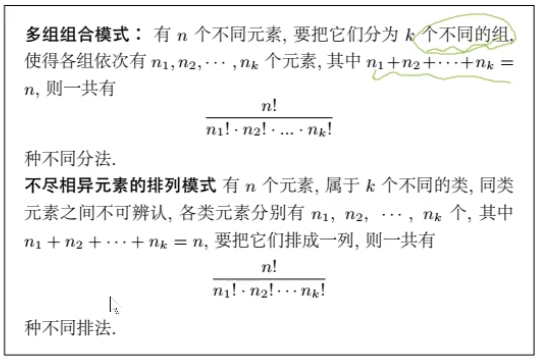
\includegraphics[scale=0.6]{multi-combination.png}
		\end{figure}\par
	\end{itemize}
\end{itemize}

\subsubsection{古典概型}
\begin{itemize}
	\itemblt 例题
	\begin{enumerate}
		\item n男m女排圈, 女不邻. 问排法.\\
		\ovalboxn{
			解: 找一个男生为队首, 插入女生在前n个空位(插入到最后和最前是一样的), 再绕成圈.\\  这时有$|A|=(n-1)!\comb{n}{m}m!$种.\\
			再除以$|\Omega|=\frac{(n+m)!}{(m+n)}$即可.\\
			最后答案: $\comb{n}{m}/\comb{n+m-1}{m}$\\
		}
	
		\item 火柴盒问题. 2个火柴盒, 每个有n根. 每次随机拿一个盒的一根, 某次发现空了. 求此时另一盒中有m根的概率.\\
		\ovalboxn{解: $|\Omega|=2^{2n-m+1}, |A|=2\cdot\comb{2n-m}{n}$}
		
		\item 21本书分给17人. 6人0本, 5人1本, 2人2本, 4人3本.\\
		\ovalboxn{
			$|A|=\frac{17!}{6!5!2!4!}\frac{21!}{(0!)^6(1!)^5(2!)^2(3!)^4}$\\
			$|\Omega|=17^21$
		}
	\end{enumerate} 
\end{itemize}

\subsubsection{几何概型}
$P(A)=\frac{m(A)}{m(\Omega)}$
\begin{figure}[H]
	\centering
	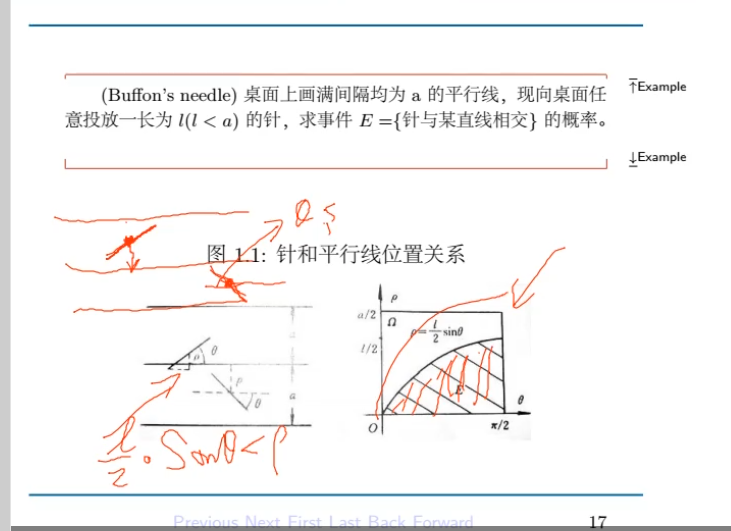
\includegraphics[scale=0.5]{Buffon.png}
\end{figure}\par

\subsection{条件概率}
\subsubsection{乘法定理}
$P(AB)=P(A|B)P(B)$
$P(A_1A_2\cdots A_n)=P(A_1)P(A_2|A_1)\cdots P(A_n|A_1\cdots A_{n-1})$

\subsubsection{全概率公式}
互不相容的事件$B_1,B_2,\cdots B_n$, 其中$B_i\cap B_j=\varnothing, \prod\limits_{i=1}^{n}B_i=\Omega$, 则$B_1,B_2,\cdots B_n$为样本空间的一个分割.\\
全概率公式+
$$P(A)=\sum\limits_{i=1}^{n}P(A|B_i)P(B_i)$$
证明:
$$\begin{aligned}
\sum\limits_{i=1}^{n}P(A|B_i)P(B_i)&=\sum\limits_{i=1}^{n}P(AB_i)\\
&=P(\sum\limits_{i=1}^{n}AB_i)=P(A\sum\limits_{i=1}^{n}B_i)\\
&=P(A\cdot\Omega)=P(A)
\end{aligned}$$
\begin{itemize}
	\itemblt (Polya罐子模型)罐子中有a个白球b个黑球, 每次摸出一个后连同c个同色球放回. 证明第n次取球, 取出白球概率为$\frac{a}{a+b}$\\
	\ovalboxn{
		假设第$n=k-1$次取, 概率为$\frac{a}{a+b}$, \\
		则有$P(A_k|A_2)=\frac{(a+c)}{(a+c)+b},\quad P(A_k|\overline{A_2})=\frac{(a)}{a+(b+c)}$,\\
		因此$P(A_k)=P(A_2)P(A_k|A_2)+P(\overline{A_2})P(A_k|\overline{A_2})=\frac{a}{a+b}$
	}
\end{itemize}

\subsubsection{贝叶斯公式}

\subsubsection{事件的独立性}
\begin{itemize}
	\itemblt 研究什么情况下$P(AB)=P(A)P(B)$,即$P(A|B)=P(A)$,$B$对$A$发生的概率没有影响, 这个和$A$对$B$发生概率没有影响是同时的.即$A$和$B$应该说是\textbf{相互}独立的.\\
	要证明$A$和$B$相互独立,只需要证明$P(\tilde{A}\tilde{B})=P(\tilde{A})P(\tilde{B})$四个式子中的一个.
	
	\itemblt 推广到$n$个事件.(以下两个定义是等价的)\\
	定义1: 只要证明$P(\tilde{A}_1\tilde{A}_2\cdots P(\tilde{A}_n)=P(\tilde{A}_1)P(\tilde{A}_2)\cdots P(\tilde{A}_n)$这$2^n$个等式都要成立.\\
	定义2: 对$A_1,\cdots A_n$中任意$k$个事件$A_{i_1},A_{i_2},\cdots,A_{i_k}$有$$P(\tilde{A}_{i_1}\tilde{A}_{i_2}\cdots P(\tilde{A}_{i_n})=P(\tilde{A}_{i_1})P(\tilde{A}_{i_2})\cdots P(\tilde{A}_{i_n})$$
	若$A_1,\cdots A_n$任意两个事件相互独立,则称为两两独立.(即k=2)
\end{itemize}


\begin{figure}[H]
	\centering
	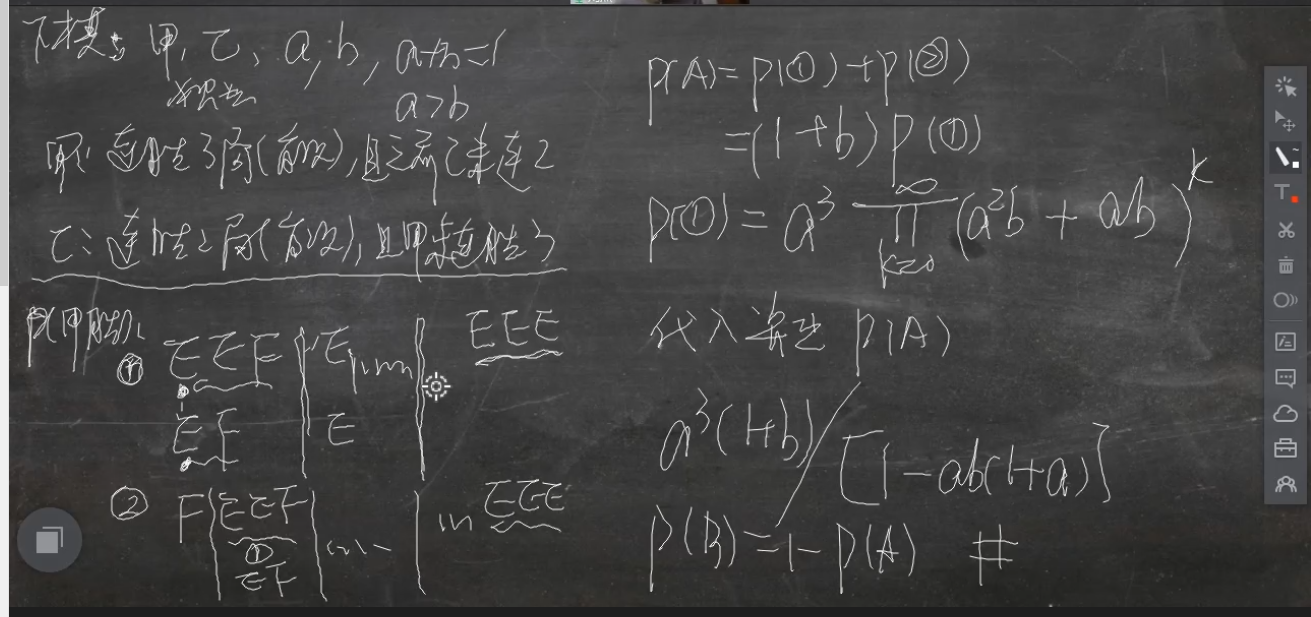
\includegraphics[scale=0.4]{2020_3_3_1.png}
\end{figure}\par

\subsection{本章小结}
\begin{itemize}
	\itemblt 古典概型/几何概型/事件运算, 排列组合
	\itemblt 独立性, 相互/两两; 应用
	\itemblt 全概率(based on 条件概率)
	\itemblt Bayes公式
\end{itemize}


\section{第二章}

\subsection{随机变量的概念}
\begin{itemize}
	\itemblt 一维: 离散,连续
	\itemblt 多维: 联合分布, 边缘分布, 条件分布密度
\end{itemize}

\subsection{离散型随机变量}
\begin{itemize}
	\itemblt 概率(质量)函数: $p_i=P(X=a_i),\ i=1,2,\cdots$
	\itemblt 分布函数:$F(x)=P(X\le x)=\sum\limits_{i:p_i\le x}P(X=a_i)=\sum\limits_{i:p_i\le x}p_i$
	\itemblt 概率函数和分布函数是一一对应的:\\
	$P(x=a_i)=P(a_{i-1}< X\le a_i)=F(a_i)-F(a_{i-1})$
	\itemblt 分布表
	\itemblt Bernoulli试验, 将一个可能结果为$A$和$\overline{A}$的Bernoulli试验独立地重复$n$次, 使得事件$A$每次出现的概率相同
\end{itemize}


\subsubsection{0-1分布}
随机变量$X$只能取$0,1$两个值, 且有
$$P(X=1)=p, P(X=0)=1-p$$
则称$X$服从0-1分布或Bernoulli分布.
\subsubsection{二项分布}
二项分布为:
$$P(X=k)=\comb{n}{k}p^k(1-p)^{n-k},\ k=0,1,\cdots,n$$
称X服从二项分布, 记为$X\sim B(n,p)$
如果$np_n\rightarrow \lambda>0$,因此$p_n\rightarrow 0$, 从而
$$\comb{n}{k}p^k(1-p)^{n-k}=\frac{1}{k!}\frac{n(n-1)\cdots(n-k+1)}{n^k}(np_n)^k(1-p_n)^n(1-p_n)^{-k}\rightarrow\frac{1}{k!}\lambda^ke^{-\lambda}$$

\subsubsection{几何分布(Geometric distribution)}
\begin{itemize}
	\itemblt 在$n$重贝努里试验中, 当$n\rightarrow \infty$, 称为\textbf{可列重贝努里试验}
	\itemblt 几何分布描述首次出现成功:
	$$P(X=k)q^{k-1}p,\ k=1,2,\cdots$$
	记为$X\sim G(p)$
	\itemblt 无记忆性!
	\itemblt $\xi$服从几何分布$G(p)$当且仅当对任何正整数$m,n$,有
	$$P(\xi>m+n|\xi>m)=P(\xi>n)$$
	这个性质成为几何分布的\textbf{无记忆性}(memoryless property)
\end{itemize}
\begin{figure}[H]
	\centering
	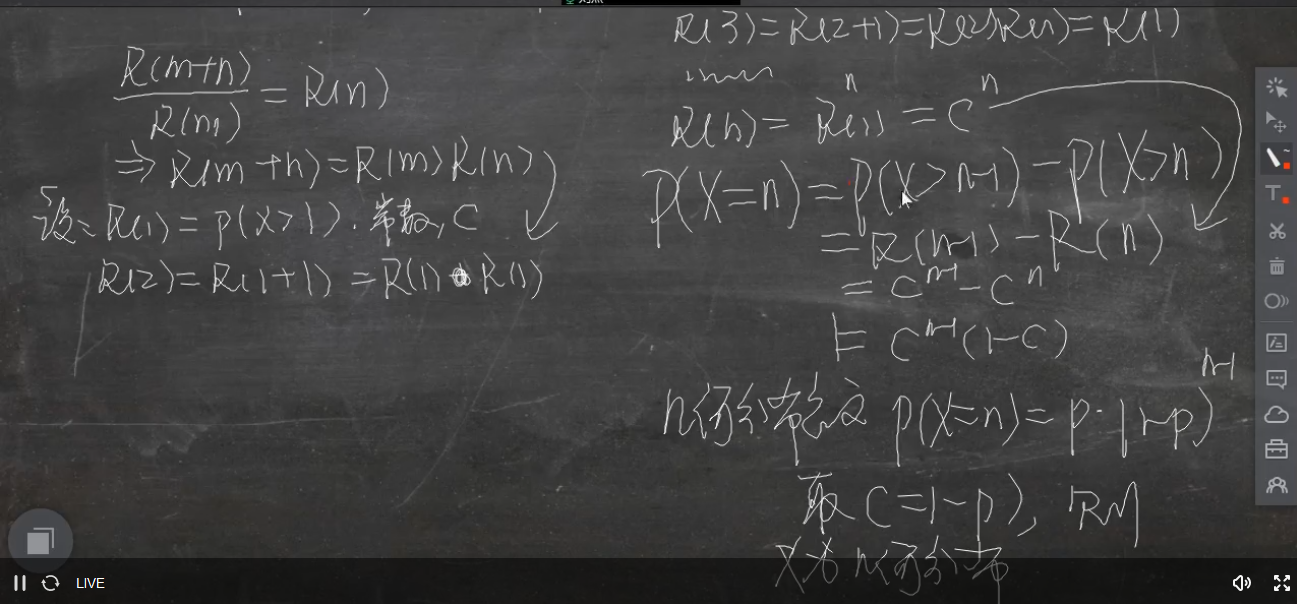
\includegraphics[scale=0.4]{2020_3_3_2.png}
\end{figure}\par

\subsubsection{Pascal分布(负二项分布)(这玩意知道就行)}
可列重贝努里试验中, 以$X_r$表示第$r$次成功发生时的试验次数, 则$X_r$的分布律为
\begin{align*}
	P(X_r=k)&=\comb{r-1}{k-1}p^{r-1}q^{k-r}p\\
	&=\comb{r-1}{k-1}p^{r-1}q^{k}\\
\end{align*}
称此概率分布为Pascal分布/负二项分布.\\
且有
$$\sum\limits_{k=r}^{\infty}p_k=p^r\sum\limits_{k=0}^{\infty}\comb{r-1}{r+k-1}q^k=p^r(1-q)^{-r}=1
$$

\subsubsection{Poisson分布}
满足
$$P(X=k)=\frac{\lambda^k}{k!}e^{-\lambda},\ k=0,1,2,\cdots,\lambda>0$$
则称$X$服从参数为$\lambda$的Poisson分布, 并记为$X\sim P(\lambda)$或$X\sim P_{oi}(\lambda)$
\begin{enumerate}
	\item 发射粒子数满足泊松分布, 接收到一个的概率为p. 最后仍然满足泊松分布$X\sim P_{oi}(p\lambda)$
\end{enumerate}


\subsubsection{离散的均匀分布}
随机变量$X$取值$a_1,a_2\cdots,a_n$
$$P(X=a_i)=\frac{1}{n}$$

\subsection{连续型随机变量}

\subsubsection{正态分布}
概率密度函数
$$f(x)=\frac{1}{\sqrt{2\pi}\sigma}\expo{-\frac{(x-\mu)^2}{2\sigma^2}}$$
记为$X\sim N(\mu, \sigma^2)$\\
标准正态分布的分布函数记为$\Phi(x)$

\subsubsection{指数分布}
概率密度函数如下
$$f(x)=\leftbig{\lambda e^{-\lambda x},\ x>0,\\0,\ x\le0}$$
其中$\lambda>0$
分布函数为
$$F(x)=\leftbig{1-e^{-\lambda x},\ x>0\\0,\ x\le0}$$
\jumpline
失效率:
$$h(x)=\lim\limits_{\Delta x\rightarrow0}\frac{P(x\le X\le x+\Delta x|X>x)}{\Delta x}$$
所以失效率最终为$h(x)\equiv\lambda,\ 0<x<+\infty$. 无记忆性.

\subsubsection{均匀分布}
设$-\infty<a<b<+\infty$, 密度函数为
$$f(x)=\leftbig{\frac{1}{b-a},\ a\le x\le b\\0,\ otherwise}$$
分布函数为
$$F(x)=\leftbig{0,\ x\le a\\\frac{x-a}{b-a},\ a<x\le b\\1,\ x>b}$$

\subsection{多维分布与边际分布}
\subsubsection{多维分布}
\begin{itemize}
	\itemblt 多项分布. $X_i$表示$A_i$出现次数, 总共$N$次.
	$$P(X_1=k_1, X_2=k_2, \cdots, X_n=k_n)=\frac{N!}{k_1!\cdots k_n!}p_1^{k_1}\cdots p_n^{k_n}$$
	记为$M(N;p_1,\cdots,p_n)$
\end{itemize}

\subsubsection{多维连续型随机变量}
\begin{itemize}
	\item 均匀分布
	$$f(x_1,x_2)=\leftbig{1/[(b-a_(d-c)],\ a\le x_1\le b, c\le x_2\le d\\0,\ otherwise}$$
	
	\item 单位圆上均匀分布
	\colorbox{yellow}{TODO}
	
	\item 二元正态分布
	$$f(x,y)=\frac{1}{2\pi\sigma_1\sigma_2\sqrt{1-\rho^2}}\expo{-\frac{1}{2(1-\rho^2)}\left[\frac{(x-a)^2}{\sigma_1^2}-2\rho\frac{(x-a)(x-b)}{\sigma_1\sigma_2}+\frac{(y-b)^2}{\sigma_2^2}\right]}$$
\end{itemize}

\subsubsection{边缘分布}

\subsubsection{条件分布和随机变量的独立性}

\subsubsection{连续型随机变量的条件分布}
有
$$f_{X|Y}(x|y)=\frac{f(x,y)}{f_Y(y)}$$

\subsection{随机变量的函数的概率分布}
$y=g(x)$严格单调连续, 反函数唯一为$x=h(y)$, 且$h'(y)$存在且连续, 则$Y=g(x)$也是连续型随机变量, 有$$p(y)=f(h(y))|h'(y)|$$

\section{大数定律和中心极限定理}
\subsection{中心极限定理}
设${X_n}$为$i.i.d.$的随机变量序列, 具有公共的数学期望$\mu$和方差$\sigma^2$, 则$X_1+\cdots+X_n$的标准化形式$\frac{1}{\sqrt{n}\sigma}(X_1+\cdots+X_n-n\mu)$满足中心极限定理, 即对任意$x\in\mathbb{R}$
$$\lim\limits_{n\rightarrow \infty}F_n(x)=\Phi(x)$$
其中$F_n(x)$是$\frac{1}{\sqrt{n}\sigma}(X_1+\cdots+X_n-n\mu)$的分布函数

\section{参数估计}
\subsection{区间估计}
\subsubsection{枢轴变量法}
\begin{enumerate}
	\item 单正态总体. $X_1, X_2, \cdots, X_n i.i.d. N(\mu, \sigma^2)$
	\begin{itemize}
		\item 估计$\mu$, 未知$\sigma$
		$$\frac{\sqrt{n}(\overline{X}-\mu)}{S}\sim t_{n-1}$$
		
		\item 估计$\sigma$, 未知$\mu$
		$$\frac{(n-1)S^2}{\sigma^2}\sim \chi_{n-1}^2$$
		
		\item 估计$\sigma$, 已知$\mu=\mu_0$.\\
		$$\sum\limits_{i=0}^n\frac{(X_i-\mu_0)^2}{\sigma^2} \sim \chi_{n}^2$$
		
		\item 估计$\mu$, 已知$\sigma=\sigma_0$
		由$\overline{X}\sim N(\mu,\frac{1}{n}\sigma_0^2)$
		有$$\frac{\overline{X}-\mu}{\sqrt{\frac{1}{n}\sigma_0^2}} \sim N(0, 1)$$
					
	\end{itemize}
	
	\item 二正态总体. $X_1, X_2, \cdots, X_m i.i.d. N(\mu_1, \sigma_1^2)$, $Y_1, Y_2, \cdots, Y_n i.i.d. N(\mu_2, \sigma_2^2)$
	\begin{itemize}
		\item 估计$\mu_1-\mu_2$, 未知$\sigma_1, \sigma_2$. \\
		根据$(\overline{X}-\overline{Y}) \sim N(\mu_1-\mu_2, \frac{1}{n}\sigma_1^2+\frac{1}{m}\sigma_2^2)$有
		$$\frac{(\overline{X}-\overline{Y})-(\mu_1-\mu_2)}{S_\omega\sqrt{\frac{m+n}{mn}}} \sim t_{n+m-2}$$
		这里$S_\omega=\frac{1}{m+n-2}(\sum\limits_{i=0}^{m}(X_i-\overline{X})+\sum\limits_{i=0}^{n}(Y_i-\overline{Y}))$
		
		\item 估计$\frac{\sigma_1}{\sigma_2}$, 未知$\mu_1, \mu_2$.\\
		根据$\frac{(n-1)S_1^2}{\sigma_1^2} \sim \chi_{n-1}^2$
		$$\frac{S_1^2}{S_2^2}\frac{\sigma_2^2}{\sigma_1^2} \sim F_{n-1, m-1}$$
		这里计算时注意$F_{n-1, m-1}(1-\frac{\alpha}{2})=1/F_{m-1, n-1}(\frac{\alpha}{2})$
		
		\item 估计$\mu_1-\mu_2$, 已知$\sigma_1=\sigma_2=\sigma_0$.
		根据$(\overline{X}-\overline{Y}) \sim N(\mu_1-\mu_2, \frac{1}{n}\sigma_1^2+\frac{1}{m}\sigma_2^2)$有
		$$\frac{(\overline{X}-\overline{Y})-(\mu_1-\mu_2)}{\sigma_0\sqrt{\frac{m+n}{mn}}} \sim N(0, 1)$$
						
		\item 估计$\frac{\sigma_1}{\sigma_2}$, 已知$\mu_1, \mu_2$.\\
		根据$\sum\limits_{i=0}^n\frac{(X_i-\mu_0)^2}{\sigma_1^2} \sim \chi_{n}^2$及$\sum\limits_{i=0}^m\frac{(Y_i-\mu_0)^2}{\sigma_2^2} \sim \chi_{m}^2$有
		$$\frac{\frac{1}{n}\sum\limits_{i=0}^n(X_i-\mu_0)^2}{\frac{1}{m}\sum\limits_{i=0}^m(Y_i-\mu_0)^2}\cdot\frac{\sigma_2^2}{\sigma_1^2} \sim F_{n, m}$$
		这里计算时注意$F_{n, m}(1-\frac{\alpha}{2})=1/F_{m, n}(\frac{\alpha}{2})$
		
	\end{itemize}
\end{enumerate}
\subsubsection{大样本法}
利用中心极限定理即可

\section{假设检验}
\begin{figure}[H]
	\centering
	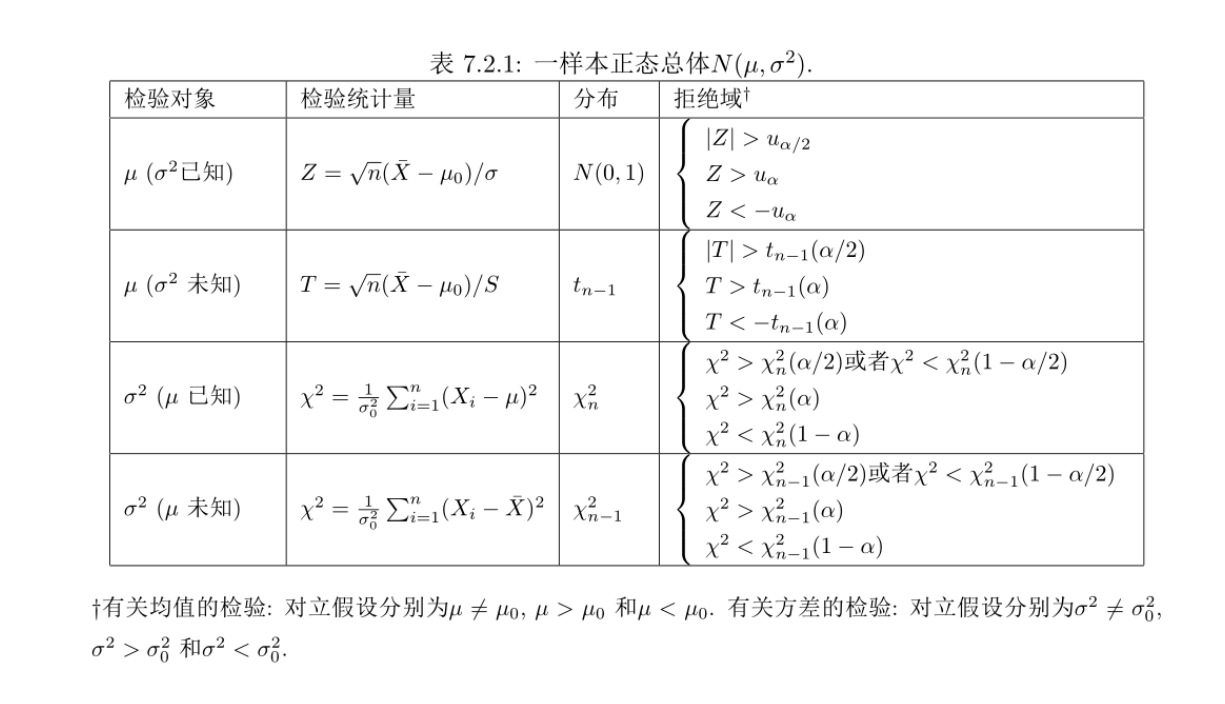
\includegraphics[width=\linewidth]{one_sample_norm.png}
\end{figure}
\begin{figure}[H]
	\centering
	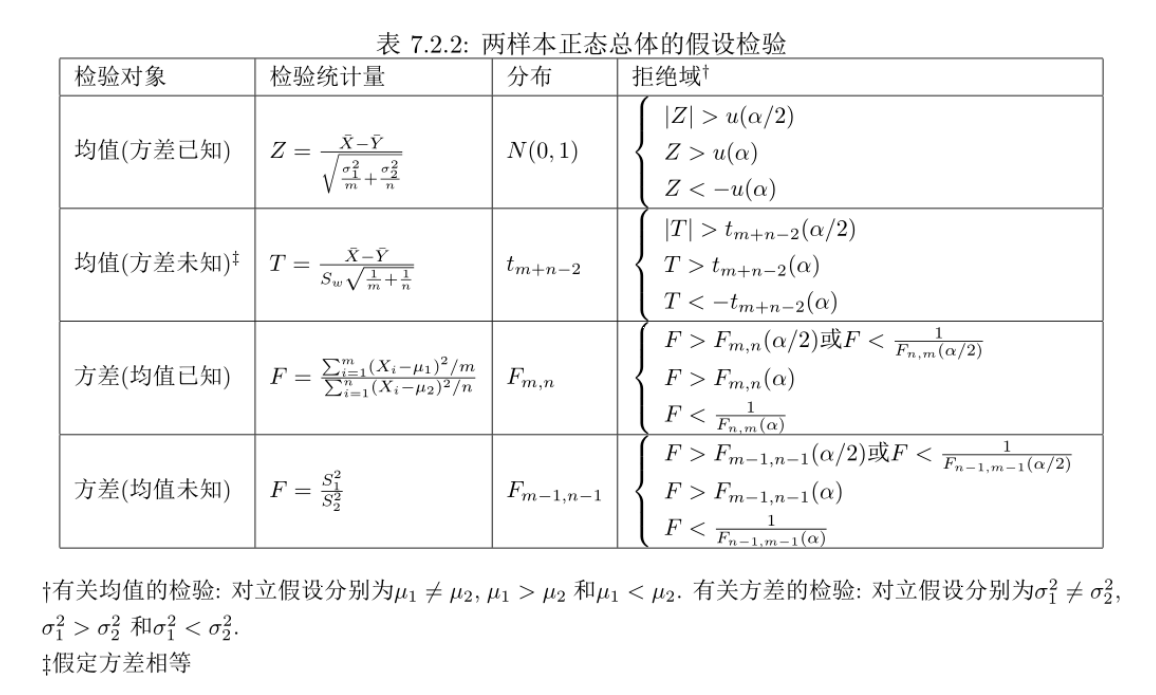
\includegraphics[width=\linewidth]{two_sample_norm.png}
\end{figure}

\end{document}



















